% Gauss: dos volúmenes adyacentes; las caras internas se cancelan (libro fig. 2.11)
\documentclass[border=5pt]{standalone}
\usepackage{tikz}
\usetikzlibrary{arrows.meta, calc}
\begin{document}
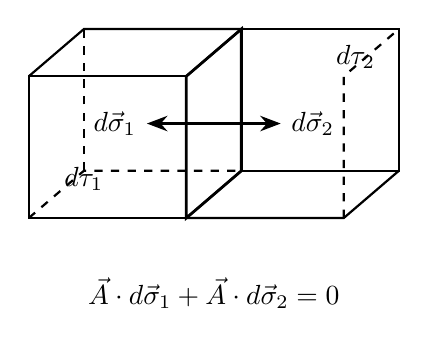
\begin{tikzpicture}[>={Stealth[length=2.6mm]}, line width=0.8pt]
  % dos cajas en perspectiva compartiendo la cara central
  % caja izquierda
  \draw (0,0)--(2,0)--(2,1.8)--(0,1.8)--cycle;
  \draw (0,1.8)--(0.7,2.4)--(2.7,2.4)--(2,1.8);
  \draw (2,0)--(2.7,0.6)--(2.7,2.4);
  \draw[dashed] (0,0)--(0.7,0.6)--(2.7,0.6); \draw[dashed] (0.7,0.6)--(0.7,2.4);
  % caja derecha (compartiendo la cara en x=2..2.7)
  \draw (2.7,0.6)--(4.7,0.6)--(4.7,2.4)--(2.7,2.4);
  \draw (4.7,0.6)--(4.0,0.0)--(2.0,0.0); \draw[dashed] (4.0,0.0)--(4.0,1.8)--(4.7,2.4);
  \draw[dashed] (2.0,0.0)--(4.0,0.0);
  % cara común y normales opuestas
  \draw[line width=1pt] (2,0)--(2.7,0.6)--(2.7,2.4)--(2,1.8)--cycle;
  \draw[->, line width=1.1pt] (2.35,1.2)--(1.5,1.2) node[left]{$d\vec\sigma_1$};
  \draw[->, line width=1.1pt] (2.35,1.2)--(3.2,1.2) node[right]{$d\vec\sigma_2$};
  \node at (2.35,-0.95){$\vec A\cdot d\vec\sigma_1+\vec A\cdot d\vec\sigma_2=0$};
  \node at (0.7,0.5){$d\tau_1$}; \node at (4.15,2.05){$d\tau_2$};
\end{tikzpicture}
\end{document}
